%
% spektral.tex -- spektrale Graphentheorie
%
% (c) 2020 Prof Dr Andreas Müller, Hochschule Rapperswil
%
\section{Spektrale Graphentheorie
\label{buch:section:spektrale-graphentheorie}}
\rhead{Spektrale Graphentheorie}
Die Adjazenz-Matrix, die Grad-Matrix und damit natürlich auch
die Laplace-Matrix codieren alle wesentliche Information eines
ungerichteten Graphen.
Sie operiert auf Vektoren, die für jeden Knoten des Graphen eine
Komponente haben.
Dies eröffnet die Möglichkeit, den Graphen über die linearalgebraischen
Eigenschaften dieser Matrizen zu studieren.
Dieser Abschnitt soll diese Idee an dem ziemlich übersichtlichen Beispiel
der chromatischen Zahl eines Graphen illustrieren.

\subsection{Chromatische Zahl und Unabhängigkeitszahl
\label{buch:subsection:chromatische-zahl}}
Der Grad eines Knotens ist ein mass dafür, wie stark ein Graph
``vernetzt'' ist.
Je höher der Grad, desto mehr direkte Verbindungen zwischen Knoten gibt es.
Noch etwas präziser können diese Idee die beiden mit Hilfe der
chromatischen zahl und der Unabhängigkeitszahl erfasst werden.

\begin{definition}
Die {\em chromatische Zahl} $\operatorname{chr}G$ eines Graphen $G$ ist
die minimale Anzahl von Farben, die Einfärben der Knoten eines Graphen
nötig sind, sodass benachbarte Knoten verschiedene Farben haben.
\index{chromatische Zahl}
\end{definition}

\begin{definition}
Eine Menge von Knoten eines Graphen heisst {\em unabhängig}, wenn 
keine zwei Knoten im Graphen verbunden sind.
Die {\em Unabhängigkeitszahl} $\operatorname{ind}G$ eines Graphen $G$
ist die maximale Anzahl Knoten einer unabhängigen Menge.
\index{Unabhängigkeitszahl}
\end{definition}

Zwischen der chromatischen Zahl und der Unabhängigkeitszahl eines Graphen
muss es einen Zusammenhang geben.
Je mehr Verbingungen es im Graphen gibt, desto grösser wird die chromatische
Zahl.
Gleichzeitig wird es schwieriger für Mengen von Knoten, unabhängig zu sein.

\begin{satz}
\label{buch:satz:chrind}
Ist $G$ ein Graph mit $n$ Knoten, dann gilt
$\operatorname{chr}G\cdot\operatorname{ind}G\ge n$.
\end{satz}

\begin{proof}[Beweis]
Eine minimale Färbung des Graphen mit $\operatorname{chr}G$ Farben
teilt die Knoten in $\operatorname{chr}G$ Mengen $V_f$ von Knoten mit
gleicher Farbe $f$ ein.
Da diese Mengen einfarbig sind, sind sie unabhängig, enthalten also
höchstens so viele Knoten, wie die Unabhängigkeitszahl erlaubt.
Die Gesamtzahl der Knoten ist also
\begin{align*}
V
&=
\bigcup_{\text{$f$ eine Farbe}} V_f
&&\Rightarrow&
n
&=
\sum_{\text{$f$ eine Farbe}} |V_f| 
\le
\sum_{\text{$f$ eine Farbe}} \operatorname{ind}G
=
(\text{Anzahl Farben})\cdot \operatorname{ind}G
\\
&
&&&
&=
\operatorname{chr}G \cdot \operatorname{ind}G
\end{align*}
Damit ist $n\le \operatorname{chr}G\cdot\operatorname{ind}G$ gezeigt.
\qedhere
\end{proof}

\begin{beispiel}
In einem vollständigen Graphen ist jeder Knoten mit jedem anderen verbunden.
Jede Menge mit zwei oder mehr Knoten kann daher nicht unabhängig sein, die
Unabhängigkeitszahl ist daher $\operatorname{ind}G=1$.
Andererseits ist für jeden Knoten eine eigene Farbe nötig, daher ist die
chromatische Zahl $\operatorname{chr}G=n$.
Die Ungleichung von Satz~\ref{buch:satz:chrind} ist erfüllt, sogar mit
Gleichheit.
Das Beispiel zeigt, dass die Ungleichung nicht ohne zusätzliche Annahmen
verbessert werden kann.
\end{beispiel}

\begin{figure}
\centering
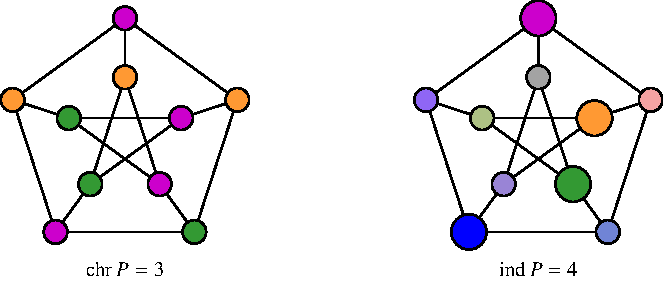
\includegraphics{chapters/70-graphen/images/petersonchrind.pdf}
\caption{Chromatische Zahl und Unabhängigkeitszahl des Peterson-Graphen.
Die chromatische Zahl ist $3$, da der Graph sich mit drei Farben einfärben
lässt (links).
Die Unabhängigkeitszahl ist $4$, die vier grösseren Knoten im rechten
Graphen sind unabhängig.
Die Farben der kleinen Knoten sind die additive Mischung der Farben
der grossen Knoten, mit denen sie verbunden sind.
\label{buch:graphen:fig:chrindpeterson}}
\end{figure}

\begin{beispiel}
Der Peterson-Graph $P$ von Abbildung~\ref{buch:graphen:fig:chrindpeterson}
hat chromatische Zahl $\operatorname{chr}P=3$ und unabhängigkeitszahl
$\operatorname{ind}P=4$.
Die Ungleichung von Satz~\ref{buch:satz:chrind} ist erfüllt, sogar als
Ungleichung: $\operatorname{chr}P\cdot\operatorname{ind}P=3\cdot 4=12>10=n$.
\end{beispiel}

Nach Definition ist Unabhängigkeitszahl ein Mass für die Grösse einer
unabhängigen Menge von Punkten.
Der Beweis von Satz~\ref{buch:satz:chrind} zeigt, dass man sich die
chromatische Zahl als ein Mass dafür, wieviele solche anabhängige 
Mengen in einem Grapehn untergebracht werden können.

\subsection{Chromatische Zahl und maximaler Grad
\label{buch:subsection:chr-und-maximaler-grad}}

\subsection{Maximaler Eigenwert von $A(G)$ maximaler Grad
\label{buch:subsection:maximaler-eigenwert}}

\subsection{$\alpha_{\text{max}}$ eines Untegraphen
\label{buch:subsection:alphamax-eines-untergraphen}}

\subsection{Chromatische Zahl und $\alpha_{\text{max}}$
\label{buch:subsection:chr-und-alpha-max}}

